\documentclass[12pt,a4paper]{report}

% --------------------------------------------------
% PACKAGES
% --------------------------------------------------

\usepackage[margin=1in]{geometry}
\usepackage{graphicx}
\usepackage{xcolor}
\usepackage{titlesec}
\usepackage{fancyhdr}
\usepackage{hyperref}
\usepackage{booktabs}
\usepackage{array}
\usepackage{longtable}
\usepackage{enumitem}
\usepackage{caption}
\usepackage{float}
\usepackage{tcolorbox}
\usepackage{tikz}
\usetikzlibrary{positioning}
\usepackage{setspace}
\usepackage{tocloft}

% --------------------------------------------------
% DOCUMENT SETTINGS
% --------------------------------------------------

\setlength{\parskip}{6pt}
\setlength{\parindent}{0pt}

\onehalfspacing

% --------------------------------------------------
% COLORS
% --------------------------------------------------

\definecolor{primaryblue}{HTML}{1F4E79}
\definecolor{darkblue}{HTML}{17365D}
\definecolor{lightblue}{HTML}{EAF2F8}
\definecolor{accentblue}{HTML}{2E75B6}
\definecolor{lightgray}{HTML}{F4F6F7}
\definecolor{darkgray}{HTML}{4A4A4A}

% --------------------------------------------------
% HYPERLINK SETTINGS
% --------------------------------------------------

\hypersetup{
    colorlinks=true,
    linkcolor=primaryblue,
    urlcolor=accentblue,
    citecolor=primaryblue,
    pdftitle={MarketMind AI Final Project Documentation}
}

% --------------------------------------------------
% CHAPTER STYLE
% --------------------------------------------------

\titleformat{\chapter}
{\normalfont\Huge\bfseries\color{primaryblue}}
{\thechapter.}{12pt}{}

\titlespacing*{\chapter}
{0pt}{0pt}{24pt}

% --------------------------------------------------
% SECTION STYLE
% --------------------------------------------------

\titleformat{\section}
{\normalfont\Large\bfseries\color{darkblue}}
{\thesection}{10pt}{}

\titleformat{\subsection}
{\normalfont\large\bfseries\color{primaryblue}}
{\thesubsection}{10pt}{}

\titleformat{\subsubsection}
{\normalfont\normalsize\bfseries\color{darkblue}}
{\thesubsubsection}{10pt}{}

% --------------------------------------------------
% HEADER AND FOOTER
% --------------------------------------------------

\pagestyle{fancy}

\fancyhf{}

\fancyhead[L]{\small\color{darkgray}MarketMind AI}
\fancyhead[R]{\small\color{darkgray}Final Project Documentation}

\fancyfoot[C]{\thepage}

\renewcommand{\headrulewidth}{0.4pt}
\renewcommand{\headrule}{\hbox to\headwidth{
    \color{primaryblue}\leaders\hrule height \headrulewidth\hfill
}}

% --------------------------------------------------
% CUSTOM SCREENSHOT PLACEHOLDER BOX
% --------------------------------------------------

\newtcolorbox{screenshotplaceholder}[2][]{
    colback=lightblue,
    colframe=primaryblue,
    coltitle=white,
    fonttitle=\bfseries,
    title=#2,
    boxrule=0.8pt,
    arc=3mm,
    #1
}

% --------------------------------------------------
% BEGIN DOCUMENT
% --------------------------------------------------

\begin{document}

% ==================================================
% TITLE PAGE
% ==================================================

\begin{titlepage}

\centering

\vspace*{1.2cm}

{\Huge\bfseries\color{primaryblue}
MARKETMIND AI
\par}

\vspace{0.3cm}

{\Large\color{darkgray}
AI-Powered Business Intelligence and Decision Support System
\par}

\vspace{1.2cm}

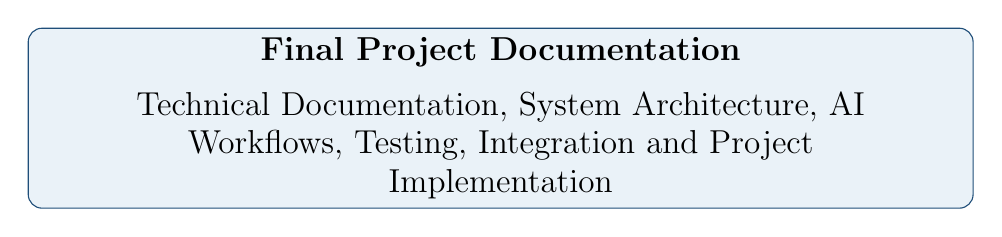
\begin{tikzpicture}
\node[
    draw=primaryblue,
    fill=lightblue,
    rounded corners=5pt,
    minimum width=12cm,
    minimum height=2cm
] {
\begin{minipage}{10.5cm}
\centering
\large
\textbf{Final Project Documentation}\\
\vspace{0.2cm}
Technical Documentation, System Architecture, AI Workflows,
Testing, Integration and Project Implementation
\end{minipage}
};
\end{tikzpicture}

\vfill

{\large\textbf{Prepared By}}
\vspace{0.3cm}

\begin{tabular}{rl}
\textbf{1.} & Damini \\[4pt]
\textbf{2.} & Pallavi \\[4pt]
\textbf{3.} & Susanna Dontha \\[4pt]
\textbf{4.} & Kavya \\[4pt]
\textbf{5.} & Pramodh \\[4pt]
\textbf{6.} & Satish
\end{tabular}

\vfill

{\large
Springboard Program
}

\vspace{0.4cm}

{\large
Final Milestone Project
}

\vspace{1cm}

{\small
\textcolor{darkgray}{September 2026}
}

\end{titlepage}

% ==================================================
% TEAM CONTRIBUTION PAGE
% ==================================================

\chapter*{Project Team}

\addcontentsline{toc}{chapter}{Project Team}

\begin{tcolorbox}[
    colback=lightgray,
    colframe=primaryblue,
    arc=3mm,
    boxrule=0.8pt,
    title=\textbf{MarketMind AI Development Team}
]

MarketMind AI was developed collaboratively by the project team.
The system integrates frontend development, backend services,
database operations, AI and machine learning modules, user
experience features, testing, and system integration.

\end{tcolorbox}

\vspace{0.5cm}

\begin{longtable}{p{0.8cm} p{3.5cm} p{8cm}}

\toprule

\textbf{No.} &
\textbf{Team Member} &
\textbf{Primary Contribution Areas}

\\

\midrule

1 &
Damini &
Application features, guided workflows, chatbot-related functionality,
authentication and additional application-level features.
\\[8pt]

2 &
Pallavi &
Frontend development, user interface implementation,
dashboards and application interface components.
\\[8pt]

3 &
Susanna Dontha &
Machine learning development with primary responsibility for
the product recommendation system, AI module development,
recommendation integration, testing, documentation and Git collaboration.
\\[8pt]

4 &
Kavya &
Machine learning and AI module development, including
collaboration on data-driven model components and ML workflows.
\\[8pt]

5 &
Pramodh &
Backend development, API integration,
system functionality and backend services.
\\[8pt]

6 &
Satish &
Backend development, integration support,
system functionality and Git-related collaboration.
\\

\bottomrule

\end{longtable}

\newpage

% ==================================================
% ABSTRACT
% ==================================================

\chapter*{Abstract}

\addcontentsline{toc}{chapter}{Abstract}

MarketMind AI is an AI-powered business intelligence and decision
support system designed to help businesses analyse customer behaviour,
business performance and operational data.

The application integrates multiple artificial intelligence and
machine learning capabilities, including customer segmentation,
forecasting, revenue analysis, churn prediction, anomaly detection
and product recommendation. The platform also includes interactive
dashboards, guided user workflows, authentication, chatbot
functionality and data-driven visualisations to support business
decision-making.

The system follows an integrated architecture consisting of a frontend
application, backend APIs, database components and machine learning
modules. Data is processed and analysed through backend services and
AI workflows, with the resulting predictions, insights and
recommendations presented through an interactive user interface.

This document presents the complete technical overview of MarketMind AI,
including the system architecture, technology stack, frontend and backend
components, AI and machine learning workflows, database integration,
application testing, system issues, solutions, limitations and future
improvements.

The report also documents the testing and integration procedures
performed during the final development phase and provides a detailed
overview of the individual modules that collectively form the
MarketMind AI platform.

\newpage

% ==================================================
% TABLE OF CONTENTS
% ==================================================

\tableofcontents

\newpage

% ==================================================
% LIST OF FIGURES
% ==================================================

\listoffigures

\newpage

% ==================================================
% LIST OF TABLES
% ==================================================

\listoftables

\newpage

% ==================================================
% CHAPTER 1
% INTRODUCTION
% ==================================================

\chapter{Introduction}

\section{Project Overview}

MarketMind AI is an AI-powered business intelligence and decision
support system developed to help businesses transform operational and
customer data into meaningful insights.

Small and medium-sized businesses often manage data related to sales,
customers, products, inventory and revenue. However, raw business data
alone does not provide sufficient support for strategic decision-making.
MarketMind AI addresses this challenge by integrating analytics,
machine learning and interactive visualisation into a unified
application.

The system provides multiple intelligent capabilities, including
customer segmentation, sales and demand forecasting, revenue analysis,
customer churn prediction, anomaly detection and personalised product
recommendations. These capabilities allow business users to identify
patterns, understand customer behaviour and receive data-driven
insights.

In addition to the AI and analytics modules, MarketMind AI includes
interactive dashboards, authentication, guided user workflows,
chatbot functionality and frontend visualisations designed to improve
the accessibility of analytical insights.

The application follows a full-stack architecture in which the frontend
communicates with backend APIs, while the backend manages database
operations, business logic and machine learning workflows. The
generated insights and predictions are returned to the frontend and
presented through interactive dashboards and user interfaces.

\begin{screenshotplaceholder}{Figure Placeholder: MarketMind AI Main Dashboard}
\centering
\vspace{1cm}

\textbf{Screenshot to Add: Main Application Dashboard}

\vspace{0.3cm}

This figure should show the primary MarketMind AI dashboard,
including business KPIs, navigation components and AI-powered
analytics modules.

\vspace{1cm}
\end{screenshotplaceholder}

\captionof{figure}{MarketMind AI Application Dashboard}
\label{fig:main-dashboard}


% ==================================================
% PROBLEM STATEMENT
% ==================================================

\section{Problem Statement}

Businesses generate large volumes of data through customer
transactions, product sales, inventory operations and revenue
activities. Although this information can contain valuable insights,
analysing it manually can be time-consuming and difficult.

Traditional dashboards primarily present historical information.
However, businesses also require intelligent systems capable of
identifying patterns, predicting future trends and generating
actionable recommendations.

The major challenges addressed by MarketMind AI include:

\begin{itemize}

    \item Difficulty in understanding customer behaviour from raw data.

    \item Limited ability to identify customer groups with similar
    purchasing patterns.

    \item Difficulty in forecasting future sales and business trends.

    \item Lack of early identification of customers who may stop
    engaging with the business.

    \item Difficulty in detecting unusual or abnormal business
    behaviour.

    \item Limited ability to generate personalised product
    recommendations.

    \item Fragmented access to business insights across multiple
    tools and data sources.

\end{itemize}

MarketMind AI addresses these challenges by providing a unified
platform that combines business analytics, machine learning models
and interactive dashboards.


% ==================================================
% PROJECT OBJECTIVES
% ==================================================

\section{Project Objectives}

The primary objective of MarketMind AI is to develop an integrated
AI-powered business intelligence platform capable of analysing
business data and generating actionable insights.

The specific objectives of the project are:

\begin{enumerate}[label=\arabic*.]

    \item To analyse customer and transactional data to identify
    meaningful behavioural patterns.

    \item To segment customers into groups based on similarities in
    purchasing behaviour and customer characteristics.

    \item To generate forecasts that can support business planning
    and decision-making.

    \item To analyse revenue-related data and present meaningful
    business performance insights.

    \item To identify customers with a higher probability of churn.

    \item To detect anomalies or unusual patterns within business
    data.

    \item To generate personalised product recommendations using
    customer behaviour and product-level signals.

    \item To provide interactive dashboards and visualisations for
    presenting analytical results.

    \item To integrate AI and machine learning workflows with a
    full-stack application architecture.

    \item To provide users with an accessible interface for exploring
    business insights and AI-generated outputs.

\end{enumerate}


% ==================================================
% PROJECT SCOPE
% ==================================================

\section{Project Scope}

MarketMind AI is designed as a business intelligence platform that
integrates multiple analytical and machine learning capabilities
within a single application.

The scope of the project includes the following major areas:

\subsection{Business Analytics}

The application provides dashboards and analytical components that
allow users to explore key business metrics and operational
information. These insights help users understand the current state
of the business and identify important patterns.

\subsection{Artificial Intelligence and Machine Learning}

The project includes multiple AI and machine learning workflows,
including:

\begin{itemize}

    \item Customer segmentation

    \item Forecasting

    \item Revenue analysis

    \item Customer churn prediction

    \item Anomaly detection

    \item Product recommendation

\end{itemize}

Each module processes available business data and generates outputs
that can support business decision-making.

\subsection{Frontend Application}

The frontend provides the primary user interface for interacting with
the system. It includes dashboards, AI module interfaces,
visualisations, navigation components and user interaction flows.

\subsection{Backend Services}

Backend services manage API requests, application logic, database
communication and integration with machine learning components.

\subsection{Database Management}

The database stores business-related information, customer data,
products, inventory records, transactions and other application data
required by the system.

\subsection{User Experience Features}

Additional application features include authentication, guided user
flows, chatbot functionality and interface components designed to
improve accessibility and user interaction.


% ==================================================
% KEY FEATURES
% ==================================================

\section{Key Features of MarketMind AI}

MarketMind AI combines multiple features within a unified
application. The major features of the system are summarised below.

\begin{table}[H]
\centering
\caption{Major Features of MarketMind AI}
\label{tab:key-features}

\begin{tabular}{p{4cm} p{9cm}}

\toprule

\textbf{Feature} &
\textbf{Description}

\\

\midrule

Interactive Dashboards &
Displays business metrics, KPIs, analytics and data-driven insights
through an interactive user interface.
\\[8pt]

Customer Segmentation &
Groups customers based on behavioural and business-related
characteristics.
\\[8pt]

Forecasting &
Generates predictions and forecasts to support future business
planning.
\\[8pt]

Revenue Analysis &
Analyses revenue-related information and business performance
patterns.
\\[8pt]

Churn Prediction &
Identifies customers who may have a higher likelihood of
disengagement or churn.
\\[8pt]

Anomaly Detection &
Detects unusual or unexpected patterns within business data.
\\[8pt]

Product Recommendation &
Generates personalised product recommendations using customer
behaviour, product signals and recommendation scoring.
\\[8pt]

Authentication &
Provides user authentication and access control for application
users.
\\[8pt]

Guided User Flow &
Helps users navigate and interact with application features through
structured workflows.
\\[8pt]

Chatbot &
Provides an additional conversational interface for user
interaction and assistance.
\\

\bottomrule

\end{tabular}

\end{table}


% ==================================================
% PROJECT VALUE
% ==================================================

\section{Business Value}

The primary value of MarketMind AI is its ability to bring together
business analytics and AI-driven insights within a unified system.

Instead of requiring users to analyse large datasets manually,
the platform provides structured analytical outputs that can support
decision-making.

The system can assist businesses in areas such as:

\begin{itemize}

    \item Understanding customer behaviour.

    \item Identifying customer segments.

    \item Monitoring business performance.

    \item Detecting unusual patterns.

    \item Identifying potential churn risks.

    \item Exploring revenue-related insights.

    \item Supporting future planning through forecasting.

    \item Discovering relevant product recommendation opportunities.

\end{itemize}

By combining these capabilities, MarketMind AI demonstrates how
machine learning and business intelligence technologies can be
integrated into a practical decision-support application.


% ==================================================
% DOCUMENT ORGANISATION
% ==================================================

\section{Document Organisation}

The remainder of this document is organised as follows:

\begin{itemize}

    \item \textbf{Chapter 2} presents the technology stack and overall
    system architecture of MarketMind AI.

    \item \textbf{Chapter 3} describes the frontend application,
    dashboards and major user-facing features.

    \item \textbf{Chapter 4} explains the backend architecture,
    APIs and database components.

    \item \textbf{Chapter 5} presents the data processing and
    machine learning workflow.

    \item \textbf{Chapter 6} describes the AI and analytics modules,
    including segmentation, forecasting, revenue analysis, churn
    prediction, anomaly detection and product recommendation.

    \item \textbf{Chapter 7} documents system integration,
    frontend-backend communication and application workflows.

    \item \textbf{Chapter 8} presents application testing,
    functional testing, integration testing and identified issues.

    \item \textbf{Chapter 9} discusses error handling and
    responsiveness improvements.

    \item \textbf{Chapter 10} documents containerisation and
    deployment status.

    \item \textbf{Chapter 11} presents challenges, limitations,
    solutions and future improvements.

    \item \textbf{Chapter 12} concludes the project and summarises
    the overall system.

\end{itemize}

\newpage
% ==================================================
% CHAPTER 1 — PROJECT INTRODUCTION
% ==================================================

\chapter{Project Introduction}

\section{Background}

Small and medium-sized businesses generate large volumes of data through
customer transactions, product sales, inventory activity and operational
processes. However, raw business data alone does not provide actionable
insights unless it is properly processed and analysed.

MarketMind AI was developed as an AI-powered business intelligence and
decision support platform to transform business data into meaningful
insights. The application combines machine learning, backend APIs,
database systems and interactive dashboards to help users understand
business performance and customer behaviour.

The platform brings together multiple analytical capabilities within a
single application. These capabilities include customer segmentation,
sales and revenue forecasting, churn prediction, anomaly detection and
product recommendations.

By integrating these modules into a unified system, MarketMind AI aims to
provide users with a centralised environment for analysing business data
and supporting data-driven decision-making.

\begin{screenshotplaceholder}{Screenshot Placeholder: MarketMind AI Application Overview}
\textbf{Suggested Screenshot:} Main application dashboard or homepage.

\vspace{0.2cm}

This screenshot should demonstrate the overall MarketMind AI interface
and provide readers with an initial visual overview of the application.
\end{screenshotplaceholder}


% ==================================================
% PROJECT PURPOSE
% ==================================================

\section{Project Purpose}

The primary purpose of MarketMind AI is to provide businesses with an
intelligent platform capable of analysing business and customer data and
generating actionable insights.

The system combines traditional business intelligence with artificial
intelligence and machine learning techniques. Instead of requiring users
to manually analyse large datasets, the application processes available
data and presents insights through dashboards, predictions and
recommendations.

The platform is designed to support several important business questions,
including:

\begin{itemize}[leftmargin=1.2cm]

\item Which customers demonstrate similar purchasing behaviour?

\item Which customers may be at risk of leaving or becoming inactive?

\item What future sales or revenue trends can be expected?

\item Are there unusual transactions or anomalies within the data?

\item Which products may be relevant for a particular customer?

\item How is the overall business performing based on available data?

\end{itemize}

By combining these analytical capabilities, MarketMind AI provides a
foundation for data-driven decision-making across multiple business
functions.


% ==================================================
% PROBLEM STATEMENT
% ==================================================

\section{Problem Statement}

Businesses often manage customer information, sales records, inventory
data and transactional information across multiple systems. Analysing
these datasets manually can be time-consuming and may make it difficult
to identify important patterns.

Several common challenges include:

\begin{itemize}[leftmargin=1.2cm]

\item Difficulty in understanding customer purchasing behaviour.

\item Limited visibility into future sales and revenue trends.

\item Difficulty identifying customers who may stop purchasing.

\item Challenges in detecting unusual transactions or abnormal patterns.

\item Difficulty identifying relevant products for individual customers.

\item Business insights distributed across multiple datasets and systems.

\end{itemize}

MarketMind AI addresses these challenges by integrating multiple
analytics and machine learning modules into a single business intelligence
platform.


% ==================================================
% PROJECT OBJECTIVES
% ==================================================

\section{Project Objectives}

The major objectives of MarketMind AI are:

\begin{enumerate}[leftmargin=1.2cm]

\item To develop an integrated business intelligence application using
frontend, backend, database and AI technologies.

\item To analyse customer and business data using machine learning
techniques.

\item To segment customers based on behavioural and transactional
characteristics.

\item To forecast business and revenue trends using available historical
data.

\item To identify potential customer churn or inactivity.

\item To detect anomalies and unusual patterns within business data.

\item To generate personalised product recommendations using customer
behaviour and product signals.

\item To provide business insights through interactive dashboards and
visualisations.

\item To integrate AI model outputs with backend APIs and frontend
components.

\item To validate system functionality through module-level, integration
and end-to-end testing.

\end{enumerate}


% ==================================================
% PROJECT SCOPE
% ==================================================

\section{Project Scope}

MarketMind AI is designed as a multi-module business intelligence
platform. The scope of the project includes the development and
integration of the following major components.

\begin{itemize}[leftmargin=1.2cm]

\item Interactive business dashboards.

\item Customer segmentation and customer analysis.

\item Forecasting and revenue analysis.

\item Customer churn prediction.

\item Anomaly detection.

\item Product recommendation functionality.

\item Guided application workflows.

\item Authentication and user-related functionality.

\item Chatbot and conversational assistance features.

\item Backend APIs and database integration.

\item Machine learning model workflows.

\item Frontend visualisation and dashboard components.

\item Functional and integration testing.

\end{itemize}

The project focuses on providing a unified platform where multiple
business analytics capabilities can be accessed through a single
application.


% ==================================================
% CHAPTER 2 — TECHNOLOGY STACK
% ==================================================

\chapter{Technology Stack}

MarketMind AI follows a full-stack architecture consisting of frontend,
backend, database and machine learning components.

The technologies used within the project support different parts of the
system, including user interface development, API services, database
operations, machine learning workflows and version control.


% ==================================================
% FRONTEND TECHNOLOGIES
% ==================================================

\section{Frontend Technologies}

The frontend is responsible for providing the user interface through
which users interact with the MarketMind AI system.

The frontend includes dashboards, analytics pages, recommendation
interfaces, data visualisations and other application screens.

\begin{table}[H]
\centering

\caption{Frontend Technology Components}

\begin{tabular}{p{4cm} p{9cm}}

\toprule

\textbf{Technology} &
\textbf{Purpose}

\\

\midrule

React &
Used for building the component-based frontend application and
interactive user interface.

\\[6pt]

JavaScript / JSX &
Used for implementing frontend logic and React components.

\\[6pt]

CSS and UI Styling &
Used for application styling, layout, responsive design and visual
presentation.

\\[6pt]

API Integration &
Used to connect frontend components with backend REST API endpoints.

\\

\bottomrule

\end{tabular}

\end{table}


% ==================================================
% BACKEND TECHNOLOGIES
% ==================================================

\section{Backend Technologies}

The backend manages business logic, API services, database communication
and integration between the frontend and machine learning modules.

\begin{table}[H]
\centering

\caption{Backend Technology Components}

\begin{tabular}{p{4cm} p{9cm}}

\toprule

\textbf{Technology} &
\textbf{Purpose}

\\

\midrule

Python &
Primary backend and machine learning programming language.

\\[6pt]

FastAPI &
Used for building backend REST APIs and handling client-server
communication.

\\[6pt]

Uvicorn &
Used as the ASGI server for running the FastAPI application.

\\[6pt]

SQLAlchemy &
Used as the ORM layer for database communication and data modelling.

\\[6pt]

Pydantic / API Schemas &
Used for request and response validation where applicable.

\\

\bottomrule

\end{tabular}

\end{table}


% ==================================================
% DATABASE TECHNOLOGIES
% ==================================================

\section{Database Technologies}

The application uses a relational database architecture to store business,
customer, product, transaction and application-related information.

\begin{table}[H]
\centering

\caption{Database Components}

\begin{tabular}{p{4cm} p{9cm}}

\toprule

\textbf{Component} &
\textbf{Purpose}

\\

\midrule

PostgreSQL &
Primary relational database used for storing application and business
data.

\\[6pt]

SQLAlchemy Models &
Represent database entities and relationships within the backend
application.

\\[6pt]

Alembic &
Database migration tool configured for managing database schema changes.

\\

\bottomrule

\end{tabular}

\end{table}


% ==================================================
% MACHINE LEARNING TECHNOLOGIES
% ==================================================

\section{Machine Learning Technologies}

The AI and machine learning layer processes business data and generates
analytical outputs such as customer segments, forecasts, churn-related
insights, anomaly detection results and product recommendations.

\begin{table}[H]
\centering

\caption{Machine Learning Components}

\begin{tabular}{p{4cm} p{9cm}}

\toprule

\textbf{Technology} &
\textbf{Purpose}

\\

\midrule

Python &
Used for machine learning development and data processing.

\\[6pt]

Pandas &
Used for structured data processing and analysis.

\\[6pt]

NumPy &
Used for numerical operations and feature processing.

\\[6pt]

Scikit-learn &
Used for machine learning workflows and predictive modelling where
applicable.

\\[6pt]

Pickle / Model Files &
Used for storing trained machine learning models and preprocessing
artifacts.

\\

\bottomrule

\end{tabular}

\end{table}


% ==================================================
% DEVELOPMENT AND COLLABORATION TOOLS
% ==================================================

\section{Development and Collaboration Tools}

The project was developed collaboratively using version control and
team-based development workflows.

\begin{table}[H]
\centering

\caption{Development and Collaboration Tools}

\begin{tabular}{p{4cm} p{9cm}}

\toprule

\textbf{Tool} &
\textbf{Purpose}

\\

\midrule

Git &
Used for source code version control and branch management.

\\[6pt]

GitHub &
Used for remote repository hosting, collaboration and code integration.

\\[6pt]

Virtual Environment &
Used to manage Python project dependencies.

\\[6pt]

PowerShell / Terminal &
Used for running backend services, Python scripts and development
commands.

\\

\bottomrule

\end{tabular}

\end{table}


% ==================================================
% TECHNOLOGY STACK SUMMARY
% ==================================================

\section{Technology Stack Summary}

The following table summarises the overall technology architecture of
MarketMind AI.

\begin{table}[H]

\centering

\caption{MarketMind AI Technology Stack}

\begin{tabular}{p{4cm} p{9cm}}

\toprule

\textbf{Layer} &
\textbf{Primary Technologies}

\\

\midrule

Frontend &
React, JavaScript, JSX, CSS

\\[6pt]

Backend &
Python, FastAPI, Uvicorn

\\[6pt]

Database &
PostgreSQL, SQLAlchemy, Alembic

\\[6pt]

Machine Learning &
Python, Pandas, NumPy, Scikit-learn

\\[6pt]

Model Storage &
Serialized model and preprocessing files

\\[6pt]

Version Control &
Git and GitHub

\\

\bottomrule

\end{tabular}

\end{table}


% ==================================================
% CHAPTER 3 — SYSTEM ARCHITECTURE
% ==================================================

\chapter{System Architecture}

MarketMind AI follows a layered full-stack architecture where the
frontend, backend, database and machine learning components work
together to deliver business intelligence functionality.

The architecture allows user requests to flow from the frontend to the
backend APIs. The backend processes requests, communicates with the
database and invokes machine learning workflows where required. The
resulting insights are returned through API responses and displayed
through the frontend.


\section{High-Level Architecture}

The high-level system architecture can be represented as follows:

\begin{center}

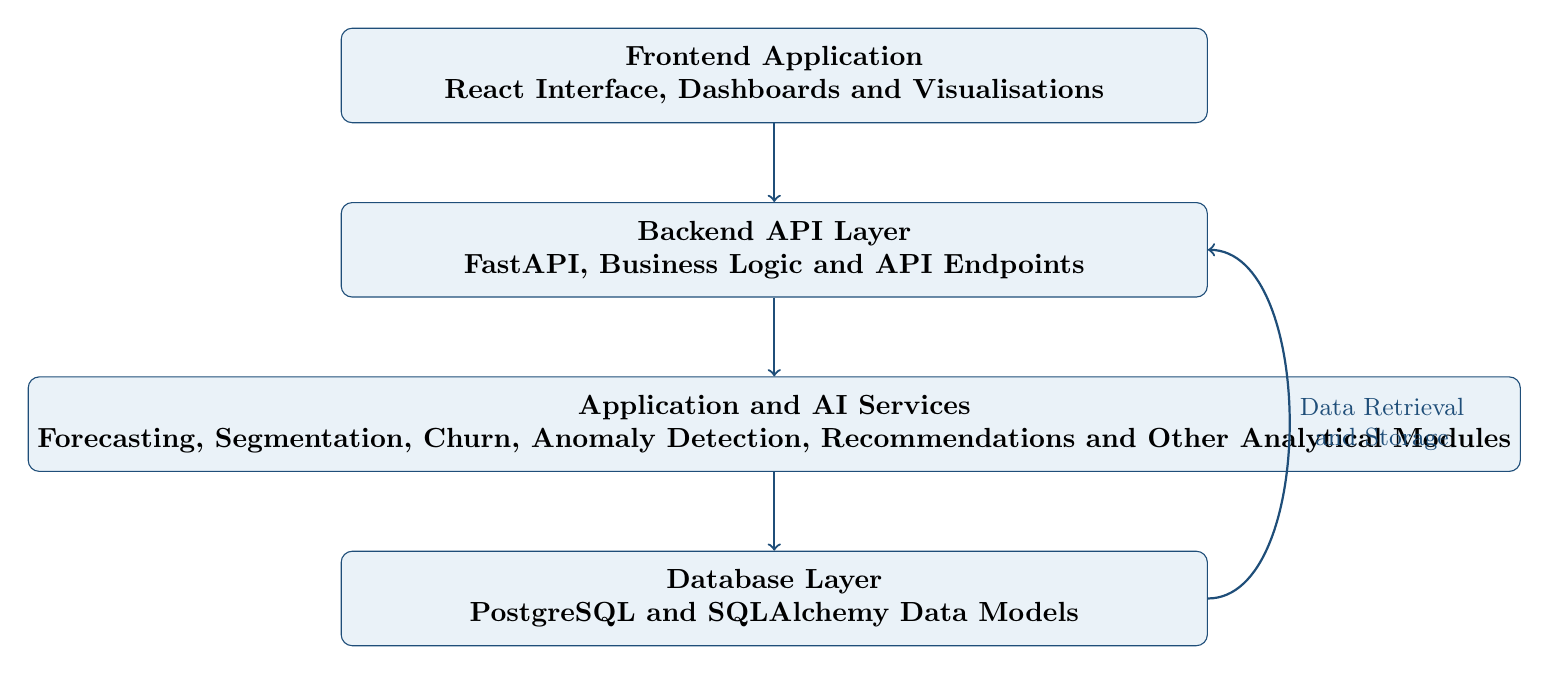
\begin{tikzpicture}[
node distance=1cm,
box/.style={
draw=primaryblue,
fill=lightblue,
rounded corners=4pt,
minimum width=11cm,
minimum height=1.2cm,
align=center,
font=\bfseries
},
arrow/.style={
->,
thick,
color=primaryblue
}
]

\node[box] (frontend)
{Frontend Application\\
React Interface, Dashboards and Visualisations};

\node[box, below=of frontend] (backend)
{Backend API Layer\\
FastAPI, Business Logic and API Endpoints};

\node[box, below=of backend] (services)
{Application and AI Services\\
Forecasting, Segmentation, Churn, Anomaly Detection,
Recommendations and Other Analytical Modules};

\node[box, below=of services] (database)
{Database Layer\\
PostgreSQL and SQLAlchemy Data Models};

\draw[arrow] (frontend) -- (backend);

\draw[arrow] (backend) -- (services);

\draw[arrow] (services) -- (database);

\draw[arrow] (database.east)
to[out=0,in=0,looseness=0.8]
node[right,align=center,font=\small]
{Data Retrieval\\and Storage}
(backend.east);

\end{tikzpicture}

\end{center}


\begin{screenshotplaceholder}{Diagram Placeholder: MarketMind AI System Architecture}
\textbf{Suggested Diagram:} Final detailed system architecture diagram.

\vspace{0.2cm}

The final diagram should visually demonstrate the relationship between
the frontend application, backend APIs, database layer and AI/ML modules.
\end{screenshotplaceholder}


% ==================================================
% ARCHITECTURE LAYERS
% ==================================================

\section{Frontend Layer}

The frontend layer provides the primary interaction point between the
user and MarketMind AI.

Users access dashboards, analytical modules and AI-generated insights
through the frontend interface. The frontend communicates with backend
API endpoints to retrieve business data and machine learning results.

Major frontend responsibilities include:

\begin{itemize}[leftmargin=1.2cm]

\item Displaying business dashboards.

\item Presenting analytics and AI outputs.

\item Displaying forecasts and revenue insights.

\item Presenting customer segmentation information.

\item Displaying churn and anomaly-related outputs.

\item Displaying personalised product recommendations.

\item Providing guided application flows and user interactions.

\item Communicating with backend APIs.

\end{itemize}


% ==================================================
% BACKEND LAYER
% ==================================================

\section{Backend Layer}

The backend acts as the central integration layer of the application.

Backend APIs receive requests from the frontend and coordinate access to
database information and AI workflows. The backend also transforms data
into API responses that can be consumed by frontend components.

The backend is responsible for:

\begin{itemize}[leftmargin=1.2cm]

\item Managing REST API endpoints.

\item Processing frontend requests.

\item Communicating with database models.

\item Executing application business logic.

\item Integrating machine learning workflows.

\item Returning structured responses to the frontend.

\item Supporting authentication and application-level functionality.

\end{itemize}


% ==================================================
% DATABASE LAYER
% ==================================================

\section{Database Layer}

The database layer stores the structured information required by the
application.

Database entities support business operations and AI workflows by storing
information related to customers, products, transactions, inventory and
other application data.

The SQLAlchemy ORM layer provides Python-based representations of
database tables and relationships.

The database also supports AI modules by providing historical and
transactional data required for analytical workflows.


% ==================================================
% AI AND MACHINE LEARNING LAYER
% ==================================================

\section{AI and Machine Learning Layer}

The AI and machine learning layer provides the analytical intelligence of
MarketMind AI.

Different modules process available business and customer data to generate
insights and predictions.

The major analytical components include:

\begin{itemize}[leftmargin=1.2cm]

\item Customer segmentation.

\item Forecasting.

\item Revenue analysis.

\item Customer churn analysis.

\item Anomaly detection.

\item Product recommendation.

\item Conversational and chatbot functionality.

\end{itemize}

Each module follows its own data processing and prediction workflow while
remaining integrated with the backend API layer.


% ==================================================
% END-TO-END DATA FLOW
% ==================================================

\section{End-to-End Application Workflow}

The general workflow of MarketMind AI follows the sequence below.

\begin{enumerate}[leftmargin=1.2cm]

\item The user interacts with a dashboard or application feature through
the frontend.

\item The frontend sends an API request to the backend.

\item The backend validates and processes the request.

\item Relevant information is retrieved from the database.

\item If required, the backend invokes the appropriate AI or machine
learning workflow.

\item The AI module processes the available data and generates an output.

\item The backend prepares the result as a structured API response.

\item The frontend receives the response.

\item The result is displayed through dashboards, charts, cards,
tables or analytical components.

\end{enumerate}


\begin{screenshotplaceholder}{Diagram Placeholder: End-to-End MarketMind AI Workflow}
\textbf{Suggested Diagram:} User $\rightarrow$ Frontend $\rightarrow$ API
$\rightarrow$ Database / AI Module $\rightarrow$ API Response
$\rightarrow$ Dashboard.

\vspace{0.2cm}

This diagram should demonstrate the complete flow of information through
the MarketMind AI application.
\end{screenshotplaceholder}


% ==================================================
% ARCHITECTURE BENEFITS
% ==================================================

\section{Architecture Benefits}

The layered architecture provides several advantages for the application.

\begin{itemize}[leftmargin=1.2cm]

\item Clear separation between frontend, backend, database and AI
components.

\item Easier integration of multiple machine learning modules.

\item Improved maintainability and modular development.

\item Independent development of frontend and backend components.

\item Easier testing of APIs and machine learning workflows.

\item Ability to extend the platform with additional AI modules.

\item Structured integration between business data and analytical
workflows.

\end{itemize}

The architecture therefore supports the project's objective of combining
multiple business intelligence capabilities within a single integrated
application.


\newpage

% ==================================================
% CHAPTER 4
% SYSTEM ARCHITECTURE AND TECHNOLOGY STACK
% ==================================================

\chapter{System Architecture and Technology Stack}

\section{System Architecture Overview}

MarketMind AI follows a modular, full-stack architecture that integrates
a web-based frontend, backend API services, a relational database and
multiple Artificial Intelligence and Machine Learning modules.

The architecture is designed to support the complete flow of business
data from user interaction and data storage to machine learning analysis
and the presentation of insights through interactive dashboards.

The major layers of the system are:

\begin{itemize}[leftmargin=1.2cm]
    \item Frontend Application Layer
    \item Backend API and Business Logic Layer
    \item Database and Data Management Layer
    \item Artificial Intelligence and Machine Learning Layer
\end{itemize}

The frontend communicates with the backend through API requests.
The backend processes requests, interacts with the database and invokes
the required AI or machine learning workflows. The generated predictions,
insights, forecasts and recommendations are then returned to the frontend
and displayed to the user through dashboards and interactive interfaces.

\begin{screenshotplaceholder}{System Architecture Diagram --- MarketMind AI}
\textbf{Suggested Figure:} Insert a high-level system architecture diagram here.

\vspace{0.3cm}

The diagram should illustrate the following flow:

\begin{center}
User $\rightarrow$ React Frontend $\rightarrow$ FastAPI Backend
$\rightarrow$ Database / AI Modules
$\rightarrow$ API Response $\rightarrow$ Dashboard
\end{center}

\vspace{0.3cm}

\textbf{Recommended Caption:}
``High-Level Architecture of the MarketMind AI System''
\end{screenshotplaceholder}


\section{High-Level System Workflow}

The overall workflow of MarketMind AI can be described as follows:

\begin{enumerate}[leftmargin=1.2cm]
    \item The user interacts with the MarketMind AI frontend.
    \item The frontend sends requests to the backend API.
    \item The backend validates and processes the request.
    \item Relevant business and customer data is retrieved from the database.
    \item The appropriate AI or machine learning workflow is executed.
    \item Predictions, insights or recommendations are generated.
    \item The backend returns the processed results through API responses.
    \item The frontend displays the results through dashboards, charts,
    cards, tables and interactive interfaces.
\end{enumerate}

This architecture separates the presentation layer, business logic,
data storage and AI processing components. This separation improves
maintainability and allows individual modules to be updated or improved
without redesigning the complete application.


% ==================================================
% FRONTEND ARCHITECTURE
% ==================================================

\section{Frontend Architecture}

The frontend provides the primary user interface for interacting with
MarketMind AI. It is responsible for presenting business insights,
machine learning outputs and application features in an interactive and
user-friendly format.

The frontend includes multiple pages and dashboards that allow users to
access different areas of the application.

Key frontend responsibilities include:

\begin{itemize}[leftmargin=1.2cm]
    \item User interaction and navigation
    \item Dashboard presentation
    \item Display of charts and business visualisations
    \item Presentation of AI and machine learning outputs
    \item Customer and product insights
    \item Forecasting and prediction result display
    \item Recommendation presentation
    \item Authentication-related user interfaces
    \item Guided workflows and application navigation
    \item Error and loading state presentation
\end{itemize}

The frontend communicates with backend APIs to retrieve data and
machine learning results. API responses are processed and displayed
through reusable interface components.

\subsection{Dashboard and Visualisation Layer}

The dashboard layer provides a central interface for analysing business
performance and AI-generated insights.

Depending on the available module, the application presents information
through:

\begin{itemize}[leftmargin=1.2cm]
    \item Summary metric cards
    \item Interactive charts
    \item Customer analysis views
    \item Revenue insights
    \item Forecasting outputs
    \item Churn-related insights
    \item Anomaly detection results
    \item Product recommendations
    \item Data tables and detailed views
\end{itemize}

The purpose of the dashboard layer is to convert raw business and model
outputs into information that can be understood and used for
decision-making.

\begin{screenshotplaceholder}{Frontend Dashboard Screenshots}
\textbf{Suggested Figures:}

\vspace{0.2cm}

Insert screenshots of the following interfaces:

\begin{itemize}
    \item Main Dashboard
    \item AI Insights or Analytics Dashboard
    \item Customer Analytics
    \item Product Recommendation Dashboard
\end{itemize}

\vspace{0.2cm}

\textbf{Recommended Caption:}
``MarketMind AI Frontend Dashboard and Analytics Interfaces''
\end{screenshotplaceholder}


% ==================================================
% BACKEND ARCHITECTURE
% ==================================================

\section{Backend Architecture}

The backend acts as the central processing layer of the MarketMind AI
application. It manages API requests, database communication,
application logic and integration with machine learning workflows.

The backend is responsible for connecting the frontend, database and AI
components into a unified application workflow.

The major backend responsibilities include:

\begin{itemize}[leftmargin=1.2cm]
    \item API request handling
    \item Authentication and user-related functionality
    \item Database communication
    \item Business logic processing
    \item AI and machine learning workflow integration
    \item Data retrieval and processing
    \item Recommendation generation and retrieval
    \item Forecasting and analytical workflows
    \item Error handling
    \item API response generation
\end{itemize}

The backend is structured using modular application components. This
allows individual functional areas to be organised into dedicated routes,
services and machine learning modules.

\subsection{API and Router Structure}

The application uses API routes to connect the frontend with backend
functionality.

Different functional areas are handled through dedicated routes and
modules. These routes process incoming requests and return structured
responses to the frontend.

The API layer enables the frontend to access:

\begin{itemize}[leftmargin=1.2cm]
    \item Business data
    \item Customer information
    \item Product information
    \item AI-generated predictions
    \item Forecasting results
    \item Churn analysis
    \item Anomaly detection results
    \item Product recommendations
    \item Dashboard analytics
\end{itemize}


% ==================================================
% DATABASE ARCHITECTURE
% ==================================================

\section{Database Architecture}

MarketMind AI uses a relational database architecture to store and
manage business, customer, product and application data.

The database acts as the central data layer for both the application and
the AI workflows. Backend services retrieve and process this data before
passing relevant information to machine learning modules.

The system uses SQLAlchemy as the Object Relational Mapping (ORM) layer
to interact with the database through Python models.

The database supports core application entities such as:

\begin{itemize}[leftmargin=1.2cm]
    \item Users
    \item Customers
    \item Products
    \item Categories
    \item Orders and transactions
    \item Inventory
    \item Business-related records
    \item Recommendation records
    \item Application and authentication-related data
\end{itemize}

The relational structure enables the application to connect customers,
products, transactions and inventory information for business analysis
and AI processing.

\subsection{Database and AI Integration}

The AI modules retrieve the required historical and behavioural data
from the database.

For example, customer and transaction data can be used for customer
segmentation, churn analysis and product recommendations, while
historical business data can support forecasting and anomaly detection
workflows.

The general integration flow is:

\begin{center}
Database $\rightarrow$ Data Processing $\rightarrow$ AI Model
$\rightarrow$ Generated Output $\rightarrow$ API $\rightarrow$ Frontend
\end{center}

\begin{screenshotplaceholder}{Database Architecture or ER Diagram}
\textbf{Suggested Figure:} Insert a simplified Entity Relationship Diagram
(ER Diagram) or database architecture diagram.

\vspace{0.2cm}

The diagram may include relationships between:

\begin{itemize}
    \item Customers
    \item Orders / Transactions
    \item Products
    \item Categories
    \item Inventory
    \item Product Recommendations
\end{itemize}

\vspace{0.2cm}

\textbf{Recommended Caption:}
``Simplified Database Architecture of MarketMind AI''
\end{screenshotplaceholder}


% ==================================================
% AI AND ML ARCHITECTURE
% ==================================================

\section{AI and Machine Learning Architecture}

The Artificial Intelligence and Machine Learning layer is responsible
for analysing business data and generating predictive and analytical
insights.

MarketMind AI integrates multiple AI and machine learning modules rather
than relying on a single model. Each module addresses a different
business problem and contributes to the overall decision support
capabilities of the platform.

The major AI and analytical components include:

\begin{enumerate}[leftmargin=1.2cm]
    \item Customer Segmentation
    \item Forecasting
    \item Revenue Analysis
    \item Churn Prediction
    \item Anomaly Detection
    \item Product Recommendation System
    \item AI Assistant and Chatbot Functionality
\end{enumerate}

These modules process available business and customer data to generate
different types of outputs such as customer groups, future predictions,
revenue insights, risk indicators, anomaly alerts and personalised
product recommendations.

\subsection{AI Module Workflow}

Although each AI module uses its own workflow, the general architecture
follows a similar pattern:

\begin{center}
Business Data
$\rightarrow$
Data Processing
$\rightarrow$
Feature Preparation
$\rightarrow$
AI / ML Model
$\rightarrow$
Prediction or Insight
$\rightarrow$
API Response
$\rightarrow$
Frontend Visualisation
\end{center}

This modular approach allows each analytical workflow to operate
independently while remaining integrated into the overall MarketMind AI
platform.


% ==================================================
% AI MODULES OVERVIEW
% ==================================================

\section{AI Module Overview}

\subsection{Customer Segmentation}

The customer segmentation module analyses customer-related information
and groups customers based on behavioural or business-related patterns.

Segmentation helps businesses understand different customer groups and
supports more targeted decision-making.

The generated customer segments can be used to support:

\begin{itemize}[leftmargin=1.2cm]
    \item Customer analysis
    \item Marketing strategies
    \item Customer behaviour understanding
    \item Personalised business decisions
\end{itemize}


\subsection{Forecasting}

The forecasting module analyses historical business data to estimate
future trends and values.

Forecasting can support business planning by providing insights into
possible future patterns based on historical observations.

Potential forecasting outputs include:

\begin{itemize}[leftmargin=1.2cm]
    \item Future sales trends
    \item Business performance estimates
    \item Historical trend analysis
    \item Forecast visualisations
\end{itemize}


\subsection{Revenue Analysis}

The revenue analysis functionality processes business and transaction
information to generate insights related to revenue performance.

The purpose of this module is to help users understand revenue trends,
business performance and data-driven financial insights.


\subsection{Churn Prediction}

The churn prediction module analyses customer-related data to identify
customers who may be at risk of becoming inactive or disengaging from
the business.

The module supports proactive business strategies by allowing users to
identify potential risk patterns and take action when appropriate.

Churn-related insights may be presented through:

\begin{itemize}[leftmargin=1.2cm]
    \item Customer risk indicators
    \item Churn prediction results
    \item Customer behaviour metrics
    \item Risk-related analytics
\end{itemize}


\subsection{Anomaly Detection}

The anomaly detection module analyses business data to identify unusual
patterns or observations.

Anomalies can represent unexpected changes in business behaviour,
transactions or other data patterns that may require further
investigation.

The module supports:

\begin{itemize}[leftmargin=1.2cm]
    \item Identification of unusual data patterns
    \item Detection of unexpected business activity
    \item Alert generation
    \item Analytical investigation
\end{itemize}


\subsection{Product Recommendation System}

The product recommendation system generates personalised product
suggestions using customer behaviour, purchasing history, product
signals and business-related data.

The recommendation workflow considers multiple signals where relevant,
including customer behaviour patterns, collaborative relationships,
product popularity and price compatibility.

The system also filters products based on availability and ranking
criteria before returning the final recommendations.

A detailed technical explanation of the Product Recommendation System,
including recommendation signals, ranking, filtering, fallback logic,
API integration and frontend presentation, is provided in the dedicated
AI module chapter of this document.


\subsection{AI Assistant and Chatbot}

The application also includes AI assistant and chatbot-related
functionality to support user interaction with the platform.

The chatbot provides an additional interface through which users can
interact with application features and receive assistance.

The guided workflow and chatbot functionality improve accessibility by
helping users navigate and interact with the MarketMind AI platform.


% ==================================================
% TECHNOLOGY STACK
% ==================================================

\section{Technology Stack}

MarketMind AI is developed using a modern full-stack architecture that
combines web technologies, backend services, relational databases and
machine learning tools.

\begin{longtable}{p{3.5cm} p{4cm} p{5cm}}

\toprule

\textbf{Layer} &
\textbf{Technology} &
\textbf{Purpose}

\\

\midrule

Frontend &
React / JavaScript &
Development of the web interface, dashboards and interactive
application components.
\\[6pt]

Backend &
Python / FastAPI &
API development, backend processing, business logic and AI integration.
\\[6pt]

Database &
PostgreSQL &
Storage and management of application, customer, product and business data.
\\[6pt]

ORM &
SQLAlchemy &
Database interaction using Python models and relational mappings.
\\[6pt]

Machine Learning &
Python-based ML Libraries &
Data processing, machine learning workflows and predictive analytics.
\\[6pt]

Data Processing &
Python Data Processing Tools &
Data transformation, preparation and analytical workflows.
\\[6pt]

Version Control &
Git and GitHub &
Source code management, collaboration, branch management and integration.
\\[6pt]

Containerisation &
Docker (Planned / Not Yet Deployed) &
The project was prepared for deployment-related work, but final
containerisation and cloud deployment were not completed during the
current development phase.
\\

\bottomrule

\end{longtable}


% ==================================================
% ARCHITECTURE SUMMARY
% ==================================================

\section{Architecture Summary}

MarketMind AI combines multiple system layers into a unified business
intelligence platform.

The frontend provides an interactive environment where users can access
dashboards, insights and AI-generated outputs. The backend manages API
communication, business logic and integration between the application
and machine learning modules. The database stores the structured data
required by the system, while the AI layer processes this information to
generate predictions, insights and recommendations.

The modular architecture allows MarketMind AI to support multiple
analytical capabilities within a single application while maintaining
separation between the user interface, backend services, data storage
and AI workflows.

This architecture also provides a foundation for future improvements
such as model enhancement, expanded datasets, improved deployment
infrastructure and additional business intelligence features.

\newpage





% ==================================================
% CHAPTER 5
% ARTIFICIAL INTELLIGENCE AND MACHINE LEARNING MODULES
% ==================================================

\chapter{Artificial Intelligence and Machine Learning Modules}

\section{Overview}

MarketMind AI integrates multiple Artificial Intelligence (AI) and
Machine Learning (ML) capabilities to transform business and customer
data into actionable insights.

The platform includes the following major analytical modules:

\begin{itemize}[leftmargin=1.2cm]
    \item Customer Segmentation
    \item Forecasting
    \item Revenue Analysis
    \item Churn Prediction
    \item Anomaly Detection
    \item Product Recommendation System
    \item AI Assistant and Chatbot Functionality
\end{itemize}

Each module performs a specific analytical task and is integrated with
the backend APIs and frontend dashboards.

\begin{screenshotplaceholder}{MarketMind AI Module Overview}
\textbf{Suggested Figure:} Add a screenshot showing the major AI and
analytics modules available in the application.

\textbf{Caption:} ``AI and Machine Learning Capabilities of MarketMind AI''
\end{screenshotplaceholder}


% ==================================================
% 5.1 CUSTOMER SEGMENTATION
% ==================================================

\section{Customer Segmentation}

The Customer Segmentation module analyses customer-related data and
groups customers with similar behavioural or business characteristics.

The generated customer groups can support targeted strategies,
customer analysis and improved understanding of different customer
profiles.

\textbf{Workflow:}

\begin{center}
Customer Data
$\rightarrow$
Feature Processing
$\rightarrow$
Segmentation Model
$\rightarrow$
Customer Groups
$\rightarrow$
Dashboard
\end{center}

\begin{screenshotplaceholder}{Customer Segmentation}
\textbf{Suggested Figure:} Add a screenshot of the segmentation
dashboard or generated customer groups.

\textbf{Caption:} ``Customer Segmentation Analysis''
\end{screenshotplaceholder}


% ==================================================
% 5.2 FORECASTING
% ==================================================

\section{Forecasting}

The Forecasting module analyses historical business data to estimate
future trends and expected values.

The generated forecasts can support business planning, trend analysis
and future performance estimation.

\textbf{Workflow:}

\begin{center}
Historical Data
$\rightarrow$
Data Processing
$\rightarrow$
Forecasting Model
$\rightarrow$
Predictions
$\rightarrow$
Visualisation
\end{center}

\begin{screenshotplaceholder}{Forecasting Module}
\textbf{Suggested Figure:} Add a screenshot showing historical trends
and forecasting results.

\textbf{Caption:} ``MarketMind AI Forecasting Output''
\end{screenshotplaceholder}


% ==================================================
% 5.3 REVENUE ANALYSIS
% ==================================================

\section{Revenue Analysis}

The Revenue Analysis module processes transaction and business data to
provide insights into revenue performance and trends.

The module helps users monitor historical revenue patterns and identify
changes in business performance.

\textbf{Workflow:}

\begin{center}
Transaction Data
$\rightarrow$
Revenue Aggregation
$\rightarrow$
Trend Analysis
$\rightarrow$
Insights
$\rightarrow$
Dashboard
\end{center}

\begin{screenshotplaceholder}{Revenue Analysis}
\textbf{Suggested Figure:} Add a screenshot of the revenue dashboard
or revenue trend visualisation.

\textbf{Caption:} ``Revenue Performance Analysis''
\end{screenshotplaceholder}


% ==================================================
% 5.4 CHURN PREDICTION
% ==================================================

\section{Churn Prediction}

The Churn Prediction module analyses customer-related information to
identify customers who may be at risk of becoming inactive or
disengaging from the business.

The module supports proactive customer retention by identifying
potential risk patterns.

\textbf{Workflow:}

\begin{center}
Customer Data
$\rightarrow$
Feature Processing
$\rightarrow$
Churn Model
$\rightarrow$
Risk Prediction
$\rightarrow$
Frontend Insights
\end{center}

\subsection{Relationship with Recommendations}

Churn Prediction and the Product Recommendation System are currently
implemented as separate modules.

The recommendation workflow does not currently use churn prediction as
a direct recommendation signal. Instead, recommendations are generated
using purchasing behaviour, collaborative signals, popularity and price
compatibility.

In future versions, churn risk could be integrated to generate
retention-oriented recommendations.

\begin{screenshotplaceholder}{Churn Prediction}
\textbf{Suggested Figure:} Add a screenshot showing churn predictions
or customer risk categories.

\textbf{Caption:} ``Customer Churn Risk Analysis''
\end{screenshotplaceholder}


% ==================================================
% 5.5 ANOMALY DETECTION
% ==================================================

\section{Anomaly Detection}

The Anomaly Detection module identifies unusual patterns or observations
within available business data.

Detected anomalies may represent unusual transactions, unexpected
behaviour or data patterns that require further investigation.

\textbf{Workflow:}

\begin{center}
Business Data
$\rightarrow$
Data Processing
$\rightarrow$
Pattern Analysis
$\rightarrow$
Anomaly Detection
$\rightarrow$
Alerts and Dashboard
\end{center}

\begin{screenshotplaceholder}{Anomaly Detection}
\textbf{Suggested Figure:} Add a screenshot showing anomaly alerts,
charts or unusual observations.

\textbf{Caption:} ``Anomaly Detection Results and Alerts''
\end{screenshotplaceholder}


% ==================================================
% 5.6 PRODUCT RECOMMENDATION SYSTEM
% ==================================================

\section{Product Recommendation System}

The Product Recommendation System generates product suggestions based
on customer purchasing behaviour and multiple recommendation signals.

The objective is to recommend relevant products while considering
business constraints such as product availability.

\subsection{Recommendation Inputs}

The recommendation workflow uses available information including:

\begin{itemize}[leftmargin=1.2cm]
    \item Customer purchase history
    \item Previously purchased products
    \item Customer spending behaviour
    \item Product popularity
    \item Product prices
    \item Available inventory
\end{itemize}


\subsection{Recommendation Signals}

The system combines multiple signals when sufficient data is available:

\begin{itemize}[leftmargin=1.2cm]

    \item \textbf{Collaborative Signal:}
    Identifies products associated with customers showing similar
    purchasing behaviour.

    \item \textbf{Association Signal:}
    Uses relationships between products that may support cross-selling.

    \item \textbf{Popularity Signal:}
    Identifies products with strong overall purchasing activity and
    supports fallback recommendations.

    \item \textbf{Price Fit Signal:}
    Compares product prices with customer spending behaviour and can
    support upselling opportunities.

\end{itemize}


\subsection{Filtering and Ranking}

Candidate products are filtered before recommendations are returned.

Products with no available inventory are excluded to prevent the system
from recommending unavailable products.

The remaining candidates are ranked according to their available
recommendation signals, and the highest-ranked products are returned.


\subsection{Fallback Strategy}

Some customers may have limited purchase history.

When personalised behavioural signals are insufficient, the system can
use broader popularity and price compatibility signals to continue
generating recommendations instead of returning empty results.


\subsection{Recommendation Types}

The system supports two primary recommendation types:

\begin{itemize}[leftmargin=1.2cm]

    \item \textbf{Cross-Sell:}
    Recommending relevant or complementary products.

    \item \textbf{Upsell:}
    Identifying higher-value product opportunities based on customer
    spending behaviour.

\end{itemize}


\subsection{Recommendation Score}

Each recommendation receives a numerical score representing its
relative ranking strength.

For frontend presentation, the score can be displayed as a
percentage-style match indicator.

\begin{center}
Score = 0.0993 $\rightarrow$ Approximately 10\% Match
\end{center}

The match percentage represents the relative strength of the
recommendation and should not be interpreted as the probability that a
customer will purchase the product.


\subsection{Recommendation Workflow}

\begin{center}
Customer Data + Product Data
\end{center}

\begin{center}
$\downarrow$
\end{center}

\begin{center}
Purchase Behaviour Analysis
\end{center}

\begin{center}
$\downarrow$
\end{center}

\begin{center}
Collaborative + Association + Popularity + Price Signals
\end{center}

\begin{center}
$\downarrow$
\end{center}

\begin{center}
Inventory Filtering
$\rightarrow$
Product Ranking
$\rightarrow$
Top Recommendations
\end{center}

\begin{center}
$\downarrow$
\end{center}

\begin{center}
FastAPI Response
$\rightarrow$
Recommendation Dashboard
\end{center}


\subsection{Recommendation Frontend}

The recommendation interface presents customer-level recommendations
along with customer statistics and product details.

The interface can display:

\begin{itemize}[leftmargin=1.2cm]
    \item Customer information and purchase statistics
    \item Recommended products
    \item Match score
    \item Cross-sell or upsell type
    \item Available inventory
    \item Recommendation explanation
    \item Recommendation signal breakdown
\end{itemize}

The frontend was redesigned during the final development phase to
improve readability and the presentation of AI-generated insights.

\begin{screenshotplaceholder}{Product Recommendation Dashboard}
\textbf{Suggested Figure:} Add the final Product Recommendation
dashboard screenshot.

\textbf{Caption:} ``AI-Powered Product Recommendation Dashboard''
\end{screenshotplaceholder}

\begin{screenshotplaceholder}{Recommendation Signal Breakdown}
\textbf{Suggested Figure:} Add the ``View Recommendation Signals''
interface showing available model signals.

\textbf{Caption:} ``Recommendation Signal Breakdown and Model Transparency''
\end{screenshotplaceholder}


% ==================================================
% 5.7 AI ASSISTANT AND CHATBOT
% ==================================================

\section{AI Assistant and Chatbot}

MarketMind AI includes chatbot and AI assistant functionality to
provide an additional interactive layer for users.

The chatbot and guided workflow features help users navigate the
application, understand available features and access business-related
information more easily.

\begin{screenshotplaceholder}{AI Assistant and Guided Workflow}
\textbf{Suggested Figure:} Add screenshots of the chatbot, AI assistant
or guided workflow features.

\textbf{Caption:} ``AI Assistant, Chatbot and Guided User Workflow''
\end{screenshotplaceholder}


% ==================================================
% AI MODULE INTEGRATION
% ==================================================

\section{AI Module Integration}

Although each AI module addresses a different business problem, they
follow a common application architecture:

\begin{center}
Data Source
$\rightarrow$
Backend Processing
$\rightarrow$
AI / ML Workflow
$\rightarrow$
Prediction or Insight
$\rightarrow$
API Response
$\rightarrow$
Frontend Dashboard
\end{center}

The integration of multiple analytical capabilities allows MarketMind AI
to provide insights related to customers, forecasting, revenue,
retention, anomalies and product recommendations.


% ==================================================
% CHAPTER SUMMARY
% ==================================================

\section{Chapter Summary}

The Artificial Intelligence and Machine Learning layer is a central
component of MarketMind AI.

The platform integrates customer segmentation, forecasting, revenue
analysis, churn prediction, anomaly detection, product recommendation
and AI assistant functionality within a single business intelligence
application.

These modules process business and customer data to generate insights,
predictions and recommendations that are delivered through backend APIs
and presented through interactive dashboards.

\newpage
% ==================================================
% CHAPTER 6
% ==================================================

\chapter{Artificial Intelligence and Machine Learning Modules}

MarketMind AI integrates multiple AI and machine learning modules to
transform business data into actionable insights. These modules analyse
customers, transactions and business performance data to support
data-driven decision-making.

The major AI capabilities implemented in the system include customer
segmentation, forecasting, revenue analysis, churn prediction, anomaly
detection, product recommendations and chatbot-based assistance.

% ==================================================
% 6.1 AI MODULE OVERVIEW
% ==================================================

\section{AI Module Overview}

The AI layer processes available business and customer data through
different analytical workflows. Each module focuses on a specific
business problem and produces outputs that can be accessed through
backend APIs and visualised on the frontend.

\begin{tcolorbox}[
    colback=lightblue,
    colframe=primaryblue,
    title=\textbf{AI Capabilities},
    arc=3mm
]

\begin{itemize}[leftmargin=0.7cm]
    \item Customer Segmentation
    \item Sales and Demand Forecasting
    \item Revenue Analysis
    \item Customer Churn Prediction
    \item Anomaly Detection
    \item Product Recommendation System
    \item AI Chatbot Assistance
\end{itemize}

\end{tcolorbox}

\begin{screenshotplaceholder}{AI Module Architecture Diagram}
Insert a diagram showing how business data flows through the backend,
machine learning modules and frontend dashboards.
\end{screenshotplaceholder}

% ==================================================
% 6.2 CUSTOMER SEGMENTATION
% ==================================================

\section{Customer Segmentation}

Customer segmentation groups customers based on behavioural and
transactional characteristics. The objective is to identify meaningful
customer groups that can support targeted marketing and business
strategies.

The segmentation workflow processes customer-related features and
assigns customers to groups based on similarities in their behaviour.

Typical insights generated by the module include:

\begin{itemize}
    \item Customer groups and segments
    \item Purchasing behaviour patterns
    \item Customer value characteristics
    \item Segment-level business insights
\end{itemize}

\begin{screenshotplaceholder}{Customer Segmentation Output}
Insert a screenshot of customer segments, cluster visualisation or
segmentation dashboard.
\end{screenshotplaceholder}

% ==================================================
% 6.3 FORECASTING
% ==================================================

\section{Forecasting}

The forecasting module analyses historical business data to estimate
future sales or business trends. Historical patterns are processed to
generate future projections that can support planning and
decision-making.

The forecasting workflow includes:

\begin{enumerate}
    \item Historical data collection
    \item Data preprocessing
    \item Time-based analysis
    \item Forecast generation
    \item Visualisation of predicted trends
\end{enumerate}

The generated forecasts are presented through the application
dashboard to help users understand expected future performance.

\begin{screenshotplaceholder}{Forecasting Dashboard}
Insert a screenshot showing historical values and forecasted trends.
\end{screenshotplaceholder}

% ==================================================
% 6.4 REVENUE ANALYSIS
% ==================================================

\section{Revenue Analysis}

The revenue analysis module evaluates business transaction data to
identify revenue patterns and performance trends.

The module supports analysis of:

\begin{itemize}
    \item Revenue trends
    \item Sales performance
    \item Product-level revenue
    \item Customer contribution
    \item Business performance over time
\end{itemize}

These insights are displayed through dashboards and visualisations,
allowing users to quickly understand important revenue patterns.

\begin{screenshotplaceholder}{Revenue Analytics Dashboard}
Insert a screenshot of revenue charts and business performance
visualisations.
\end{screenshotplaceholder}

% ==================================================
% 6.5 CHURN PREDICTION
% ==================================================

\section{Customer Churn Prediction}

The churn prediction module analyses customer behaviour to identify
customers who may be at risk of becoming inactive.

Customer-related features such as purchasing behaviour, transaction
history and engagement patterns are used to generate churn-related
predictions.

The output can help businesses identify customers who may require
retention strategies or additional engagement.

\begin{screenshotplaceholder}{Churn Prediction Dashboard}
Insert a screenshot showing churn predictions, risk categories or
customer churn analysis.
\end{screenshotplaceholder}

% ==================================================
% 6.6 ANOMALY DETECTION
% ==================================================

\section{Anomaly Detection}

The anomaly detection module identifies unusual patterns or values in
business data. These anomalies may represent unexpected changes in
sales, transactions or other measurable business behaviour.

The workflow analyses available data and highlights observations that
significantly differ from expected patterns.

Potential uses include:

\begin{itemize}
    \item Identifying unusual transactions
    \item Detecting unexpected sales patterns
    \item Highlighting abnormal business activity
    \item Supporting further investigation
\end{itemize}

\begin{screenshotplaceholder}{Anomaly Detection Results}
Insert a screenshot showing detected anomalies or abnormal data points.
\end{screenshotplaceholder}

% ==================================================
% 6.7 PRODUCT RECOMMENDATION SYSTEM
% ==================================================

\section{Product Recommendation System}

The product recommendation system generates personalised product
suggestions based on customer purchasing behaviour and available
product information.

The recommendation workflow combines multiple signals where sufficient
data is available. These include customer behaviour, collaborative
patterns, product popularity and price compatibility.

For customers with limited purchase history, the system uses fallback
recommendations to ensure useful suggestions can still be generated.

\subsection{Recommendation Inputs}

The recommendation system uses available customer, order and product
information. Important inputs include purchase history, customer order
patterns, product prices and inventory availability.

\subsection{Recommendation Signals}

The system evaluates multiple recommendation signals:

\begin{itemize}
    \item \textbf{Collaborative Signal:} Identifies products based on
    similarities between customer purchasing behaviour.

    \item \textbf{Association Signal:} Identifies products that may be
    related through purchasing patterns.

    \item \textbf{Popularity Signal:} Considers products that are
    frequently purchased across customers.

    \item \textbf{Price Fit Signal:} Evaluates how well a product price
    aligns with the customer's purchasing behaviour.
\end{itemize}

Depending on the available data, some customers may receive
recommendations using multiple signals, while customers with limited
history may primarily use fallback or popularity-based signals.

\subsection{Recommendation Ranking}

Candidate products are assigned scores based on the available
recommendation signals. Products are then ranked, and the highest
scoring suitable products are returned to the user.

The system also considers factors such as:

\begin{itemize}
    \item Previously purchased products
    \item Product availability
    \item Customer purchasing patterns
    \item Relative product price
\end{itemize}

\subsection{Recommendation Types}

Recommendations may be categorised into business-oriented types such
as:

\begin{itemize}
    \item Cross-sell recommendations
    \item Upsell opportunities
    \item Popular product recommendations
\end{itemize}

\subsection{Recommendation Explanations}

Each recommendation includes a human-readable explanation describing
why the product was suggested. The recommendation output can also
include signal information to provide additional transparency.

\subsection{Recommendation API}

The backend recommendation API retrieves generated recommendations and
returns customer-level recommendation data to the frontend.

The response includes information such as:

\begin{itemize}
    \item Customer details
    \item Recommended products
    \item Product category
    \item Product price
    \item Inventory availability
    \item Recommendation type
    \item Recommendation score
    \item Recommendation reason
    \item Recommendation signals
\end{itemize}

\subsection{Recommendation Frontend}

The recommendation dashboard presents generated recommendations through
an interactive interface. Users can view customer information,
recommended products and recommendation details.

The interface also displays recommendation-related insights and signal
information when available.

\begin{screenshotplaceholder}{Product Recommendation Dashboard}
Insert the main Product Recommendation System dashboard screenshot.
\end{screenshotplaceholder}

\begin{screenshotplaceholder}{Recommendation Signal Breakdown}
Insert a screenshot showing collaborative, popularity or other
recommendation signals.
\end{screenshotplaceholder}

% ==================================================
% 6.8 AI CHATBOT
% ==================================================

\section{AI Chatbot}

MarketMind AI also includes chatbot-based functionality to support
user interaction with the application.

The chatbot provides an additional conversational interface through
which users can interact with the system and access application
assistance.

The chatbot functionality complements the dashboards and analytical
modules by providing a more interactive user experience.

\begin{screenshotplaceholder}{AI Chatbot Interface}
Insert a screenshot of the chatbot interface and example interaction.
\end{screenshotplaceholder}

% ==================================================
% 6.9 AI MODULE DATA FLOW
% ==================================================

\section{AI Module Data Flow}

The overall AI workflow follows a common data processing architecture:

\begin{enumerate}
    \item Business and customer data is stored in the database.
    \item Backend services retrieve and process the required data.
    \item Machine learning modules perform analysis or generate
    predictions.
    \item Results are returned through backend APIs.
    \item The frontend displays predictions, insights and
    recommendations to the user.
\end{enumerate}

This architecture allows individual AI modules to operate independently
while remaining integrated with the overall MarketMind AI application.


% ==================================================
% CHAPTER 7
% SYSTEM IMPLEMENTATION AND ARCHITECTURE
% ==================================================

\chapter{System Implementation and Architecture}

\section{Overview}

MarketMind AI is designed as a full-stack business intelligence
application that integrates a frontend user interface, backend services,
database components and Artificial Intelligence and Machine Learning
modules.

The system follows a layered architecture where the frontend interacts
with backend APIs, backend services process business logic and database
operations, and AI modules generate predictions, insights and
recommendations.

\begin{center}
Frontend
$\rightarrow$
Backend APIs
$\rightarrow$
Business Logic
$\rightarrow$
Database / AI Modules
\end{center}

\begin{screenshotplaceholder}{MarketMind AI System Architecture}
\textbf{Suggested Figure:} Add the complete MarketMind AI architecture
diagram showing the frontend, backend, database and AI/ML components.

\textbf{Caption:} ``MarketMind AI High-Level System Architecture''
\end{screenshotplaceholder}


% ==================================================
% 7.1 FRONTEND ARCHITECTURE
% ==================================================

\section{Frontend Architecture}

The frontend provides the primary interface through which users interact
with MarketMind AI.

The application presents dashboards, analytics, AI-generated insights,
recommendations and other business intelligence features through an
interactive interface.

The frontend is responsible for:

\begin{itemize}
    \item Displaying business dashboards and visualisations
    \item Collecting user interactions and requests
    \item Sending requests to backend APIs
    \item Displaying predictions and AI-generated results
    \item Presenting recommendations and analytical insights
    \item Providing authentication and application navigation
\end{itemize}

The interface was improved during the final development phase to enhance
visual consistency, responsiveness and the presentation of AI outputs.


\subsection{Dashboard and User Interface}

MarketMind AI includes multiple dashboard and application pages that
present business information in an accessible format.

The dashboards provide users with visual representations of business
data, including analytics, predictions, revenue insights and customer
information.

The frontend focuses on presenting complex AI outputs in a format that
is understandable for business users.

\begin{screenshotplaceholder}{MarketMind AI Dashboard}
\textbf{Suggested Figure:} Add a screenshot of the main application
dashboard.

\textbf{Caption:} ``MarketMind AI Business Intelligence Dashboard''
\end{screenshotplaceholder}


\subsection{Recommendation Interface}

The Product Recommendation interface displays personalised product
suggestions generated by the recommendation engine.

The interface presents customer-level information along with recommended
products, recommendation types, inventory information and match scores.

Where available, users can also view the recommendation signals that
contributed to the recommendation.

\begin{screenshotplaceholder}{Recommendation User Interface}
\textbf{Suggested Figure:} Add the final Product Recommendation
dashboard screenshot.

\textbf{Caption:} ``Product Recommendation System Frontend''
\end{screenshotplaceholder}


% ==================================================
% 7.2 BACKEND ARCHITECTURE
% ==================================================

\section{Backend Architecture}

The backend manages the core business logic and acts as the connection
between the frontend, database and AI modules.

Backend services process incoming API requests, retrieve data from the
database, execute required analytical workflows and return structured
responses to the frontend.

The backend architecture includes:

\begin{itemize}
    \item API routes and endpoints
    \item Business logic
    \item Database operations
    \item AI and Machine Learning integration
    \item Data processing workflows
    \item Authentication and user-related functionality
\end{itemize}


\subsection{API Communication}

The frontend communicates with the backend through API requests.

A typical application request follows the workflow:

\begin{center}

User Action

$\downarrow$

Frontend Request

$\downarrow$

Backend API

$\downarrow$

Business Logic / AI Processing

$\downarrow$

Database Access

$\downarrow$

Structured Response

$\downarrow$

Frontend Display

\end{center}

This approach separates the user interface from backend processing and
allows individual application components to remain modular.


\subsection{AI Module Integration}

AI and Machine Learning modules are integrated into the backend
application so that model outputs can be accessed through API endpoints.

The backend is responsible for:

\begin{itemize}
    \item Retrieving required business data
    \item Preparing data for analysis
    \item Executing AI and ML workflows
    \item Processing generated outputs
    \item Returning structured responses
\end{itemize}

This allows AI functionality to be integrated with the overall
application without requiring the frontend to directly interact with
machine learning code.


% ==================================================
% 7.3 DATABASE ARCHITECTURE
% ==================================================

\section{Database Architecture}

The database stores the business, customer and application information
required by the MarketMind AI system.

The stored data supports both operational functionality and analytical
workflows.

Major categories of stored information include:

\begin{itemize}
    \item User and authentication information
    \item Customer data
    \item Product information
    \item Orders and transactions
    \item Business-related data
    \item Generated AI and analytical outputs
\end{itemize}


\subsection{Database and AI Integration}

The AI modules retrieve relevant information from the database before
performing analysis.

For example, the Product Recommendation System retrieves customer,
order and product information to generate recommendations.

The generated results can then be returned through backend APIs and
displayed through the frontend.

\begin{center}

Database

$\downarrow$

Backend Data Retrieval

$\downarrow$

AI / ML Processing

$\downarrow$

Generated Insight

$\downarrow$

API Response

$\downarrow$

Frontend Dashboard

\end{center}


\subsection{Product Recommendation Data Flow}

The recommendation system uses data from multiple sources within the
application.

The workflow includes:

\begin{enumerate}
    \item Customer data is retrieved.
    \item Customer purchase history is analysed.
    \item Product information is retrieved.
    \item Recommendation signals are calculated.
    \item Candidate products are filtered based on availability.
    \item Products are ranked.
    \item Recommendations are returned through the API.
    \item The frontend displays the generated recommendations.
\end{enumerate}


% ==================================================
% 7.4 AI AND APPLICATION INTEGRATION
% ==================================================

\section{Application Integration Architecture}

MarketMind AI integrates multiple components within a single
application workflow.

\begin{center}

User

$\downarrow$

Frontend Application

$\downarrow$

Backend API Layer

$\downarrow$

Business Logic

$\downarrow$

Database \quad + \quad AI / ML Modules

$\downarrow$

Predictions / Insights / Recommendations

$\downarrow$

Frontend Dashboard

\end{center}

The architecture enables the application to combine traditional
business data processing with machine learning and AI-driven analysis.


% ==================================================
% 7.5 ERROR HANDLING
% ==================================================

\section{Error Handling and System Reliability}

Error handling is implemented across the application to improve system
reliability and user experience.

The frontend and backend were reviewed during the final development
phase to identify issues related to data availability, API
communication and unexpected system states.

Typical error-handling considerations include:

\begin{itemize}
    \item Handling unavailable or missing data
    \item Managing API communication errors
    \item Handling invalid user input
    \item Preventing unavailable products from being recommended
    \item Handling insufficient customer history
    \item Providing fallback recommendations
\end{itemize}

The Product Recommendation System also includes fallback behaviour to
ensure recommendations can still be generated when sufficient
personalised customer data is not available.


% ==================================================
% 7.6 RESPONSIVENESS AND USER EXPERIENCE
% ==================================================

\section{Responsiveness and User Experience}

The application interface was reviewed and improved to provide a more
consistent user experience.

The final development phase included improvements related to:

\begin{itemize}
    \item Dashboard layout
    \item Recommendation interface design
    \item Visual presentation of AI insights
    \item Information hierarchy
    \item Error visibility
    \item Application usability
\end{itemize}

The goal of these improvements was to make analytical information easier
to understand while maintaining a professional and technology-focused
application design.


% ==================================================
% 7.7 VERSION CONTROL AND COLLABORATION
% ==================================================

\section{Version Control and Team Collaboration}

Git and GitHub were used to manage source code, maintain version
history and support collaboration between team members.

Different features and development tasks were managed through separate
branches before integration.

The development workflow included:

\begin{itemize}
    \item Feature-based development
    \item Branch management
    \item Code commits
    \item Pulling and pushing updates
    \item Merge operations
    \item Resolving Git-related issues
\end{itemize}

During the final development phase, Git collaboration was also used to
integrate recommendation system updates, backend changes and frontend
improvements.

\begin{screenshotplaceholder}{GitHub Repository and Branch Management}
\textbf{Suggested Figure:} Add a screenshot of the GitHub repository,
branch structure or contribution history.

\textbf{Caption:} ``Source Code Version Control and Collaboration''
\end{screenshotplaceholder}


% ==================================================
% 7.8 SYSTEM IMPLEMENTATION SUMMARY
% ==================================================

\section{System Implementation Summary}

MarketMind AI combines frontend development, backend services, database
operations and Artificial Intelligence modules into a unified business
intelligence application.

The frontend provides interactive dashboards and visualisations, while
the backend manages APIs, business logic and AI integration. The
database stores the information required by operational and analytical
workflows.

The AI modules process available data to generate predictions,
insights and recommendations, which are returned through backend APIs
and presented to users through the application interface.

This layered architecture allows MarketMind AI to provide multiple
business intelligence capabilities within a single integrated platform.

\newpage
% ==================================================
% CHAPTER 8
% TESTING AND VALIDATION
% ==================================================

\chapter{Testing and Validation}

\section{Testing Overview}

MarketMind AI was tested during the final development phase to validate
application functionality, AI module outputs, backend integration and
frontend behaviour.

Testing focused on verifying that the major workflows of the application
operate correctly and that AI-generated outputs can successfully flow
from the database and backend services to the frontend interface.

The testing process included:

\begin{itemize}
    \item Functional testing
    \item AI module testing
    \item API and backend integration testing
    \item Frontend testing
    \item End-to-end workflow testing
    \item Error and edge-case testing
\end{itemize}


% --------------------------------------------------
% 8.1 FUNCTIONAL TESTING
% --------------------------------------------------

\section{Functional Testing}

The major application features were tested to verify that expected
functionality was available and that user interactions triggered the
correct backend workflows.

The testing process covered dashboards, AI modules, data retrieval and
application-level features.

\begin{table}[H]
\centering
\caption{Functional Testing Summary}
\begin{tabular}{p{4.5cm} p{6.5cm} p{2cm}}
\toprule
\textbf{Component} &
\textbf{Testing Performed} &
\textbf{Status} \\
\midrule

Customer Segmentation &
Validated customer grouping and segmentation outputs. &
Tested \\

Forecasting &
Validated forecast generation and visual output. &
Tested \\

Revenue Analysis &
Validated revenue-related calculations and dashboard insights. &
Tested \\

Churn Prediction &
Validated churn-related outputs and customer risk analysis. &
Tested \\

Anomaly Detection &
Validated anomaly identification workflows. &
Tested \\

Product Recommendations &
Tested recommendation generation using different customer scenarios. &
Tested \\

Frontend Dashboards &
Tested data display, navigation and AI output presentation. &
Tested \\

Backend APIs &
Validated API communication and response structure. &
Tested \\

\bottomrule
\end{tabular}
\end{table}


% --------------------------------------------------
% 8.2 AI MODULE TESTING
% --------------------------------------------------

\section{AI Module Testing}

The AI and Machine Learning modules were tested using different
available customer and business data scenarios.

Testing focused on validating the overall workflow rather than only
checking whether the models produced an output.

The testing workflow included:

\begin{enumerate}
    \item Retrieving data from the database.
    \item Processing data through the relevant AI workflow.
    \item Generating predictions, insights or recommendations.
    \item Validating the returned output.
    \item Verifying backend API integration.
    \item Confirming that the frontend displayed the result correctly.
\end{enumerate}


% --------------------------------------------------
% 8.3 PRODUCT RECOMMENDATION TESTING
% --------------------------------------------------

\section{Product Recommendation Testing}

The Product Recommendation System was tested using customers with
different levels of purchase history.

This included testing customers with limited transaction history as well
as customers with a larger number of historical orders.

The tests validated:

\begin{itemize}
    \item Customer data retrieval
    \item Order history analysis
    \item Recommendation generation
    \item Product ranking
    \item Inventory filtering
    \item Recommendation type generation
    \item Recommendation signal generation
    \item API response structure
    \item Frontend recommendation display
\end{itemize}

Customers with limited historical data primarily relied on fallback
recommendation behaviour, while customers with richer purchasing
history were able to produce stronger personalised signals.

\begin{screenshotplaceholder}{Recommendation System Testing Output}
Add a screenshot of terminal output, API response or recommendation
results used during testing.

Suggested Caption: ``Product Recommendation System Testing Results''
\end{screenshotplaceholder}


% --------------------------------------------------
% 8.4 API AND INTEGRATION TESTING
% --------------------------------------------------

\section{API and Integration Testing}

Backend APIs were tested to verify that data could successfully flow
between the database, backend services, AI modules and frontend.

The following workflow was validated:

\begin{center}

Database

$\downarrow$

Backend Processing

$\downarrow$

AI / ML Workflow

$\downarrow$

API Response

$\downarrow$

Frontend Display

\end{center}

Integration testing was particularly important because MarketMind AI
combines multiple independent modules within a single application.


% --------------------------------------------------
% 8.5 END-TO-END TESTING
% --------------------------------------------------

\section{End-to-End Testing}

End-to-end testing was performed to validate complete application
workflows from user interaction to final output.

Typical workflows included:

\begin{itemize}
    \item User accesses the application.
    \item Frontend requests business or AI data.
    \item Backend processes the request.
    \item Required database information is retrieved.
    \item AI processing is executed where required.
    \item Structured results are returned.
    \item The frontend displays the final output.
\end{itemize}

This testing approach helped identify integration-related issues that
may not appear when individual modules are tested independently.


% --------------------------------------------------
% 8.6 ERROR AND EDGE-CASE TESTING
% --------------------------------------------------

\section{Error and Edge-Case Testing}

The application was also tested against scenarios where data may be
missing, limited or unavailable.

Important scenarios included:

\begin{itemize}
    \item Customers with limited purchase history
    \item Missing product information
    \item Products with unavailable inventory
    \item Empty recommendation results
    \item API communication issues
    \item Missing or incomplete data
\end{itemize}

Fallback behaviour and error handling were used where applicable to
prevent unexpected system failures.

\newpage


% ==================================================
% CHAPTER 9
% CHALLENGES, ISSUES AND SOLUTIONS
% ==================================================

\chapter{Challenges, Issues and Solutions}

\section{Overview}

During the development, integration and testing of MarketMind AI,
several technical challenges were encountered.

These challenges were related to data availability, AI module
integration, recommendation persistence, database migration management,
frontend presentation and Git collaboration.

The following table summarises key issues encountered during the final
development phase.

\begin{table}[H]
\centering
\caption{Challenges and Solutions}
\begin{tabular}{p{4cm} p{4.5cm} p{4.5cm}}
\toprule

\textbf{Challenge} &
\textbf{Issue} &
\textbf{Solution / Approach} \\

\midrule

Limited Customer Data &
Some customers had very limited purchase history, resulting in weak
personalised recommendation signals. &
Implemented fallback and popularity-based recommendation behaviour. \\[6pt]

Recommendation Signals &
Some recommendation outputs initially displayed only popularity signals. &
Tested customers with larger purchase histories to validate
collaborative recommendation behaviour. \\[6pt]

Database Migration Issue &
Alembic database version history referenced a migration that was not
available in the local migration files. &
The issue was investigated and database changes were handled carefully
to avoid blocking recommendation system development. \\[6pt]

Frontend Data Display &
Some values initially displayed as zero or were unavailable because
generated data was not being returned or persisted correctly. &
Backend responses and recommendation data handling were reviewed and
updated. \\[6pt]

Recommendation Persistence &
Generated recommendation details needed to be stored and retrieved
consistently. &
Recommendation storage logic and generated output handling were
reviewed and updated. \\[6pt]

Git Branch Management &
Feature work was developed on separate branches and required merging
into the individual development branch. &
Git branch management, merging and push operations were performed to
integrate the completed work. \\

\bottomrule

\end{tabular}
\end{table}


% --------------------------------------------------
% 9.1 DATA AVAILABILITY
% --------------------------------------------------

\section{Limited Customer Behaviour Data}

One of the major challenges in recommendation development was the
availability of sufficient customer purchase history.

Customers with very limited order history do not provide enough
behavioural information for strong collaborative recommendations.

To address this issue, the recommendation system uses fallback
strategies such as popularity-based recommendations when sufficient
personalised information is unavailable.


% --------------------------------------------------
% 9.2 RECOMMENDATION SIGNAL VALIDATION
% --------------------------------------------------

\section{Recommendation Signal Validation}

During testing, some customers produced recommendation outputs with
limited personalised signals.

Further testing using customers with larger transaction histories showed
that collaborative signals could be generated when sufficient customer
behaviour data was available.

This demonstrated the importance of testing AI systems using multiple
data scenarios rather than validating results using only a single
customer.


% --------------------------------------------------
% 9.3 DATABASE MIGRATION CHALLENGES
% --------------------------------------------------

\section{Database Migration Challenges}

A database migration issue was encountered during development when the
database version history referenced an Alembic revision that was not
available in the local migration files.

This prevented automatic migration generation from completing
successfully.

The migration issue was investigated by reviewing the database version
information and available migration files. Development work continued
using alternative approaches where appropriate to avoid unnecessary
delays while preserving existing working functionality.


% --------------------------------------------------
% 9.4 INTEGRATION CHALLENGES
% --------------------------------------------------

\section{Frontend and Backend Integration}

AI modules require coordination between multiple components.

A recommendation generated by the machine learning workflow must be
correctly processed, stored or returned by the backend before it can be
displayed by the frontend.

During development, API response structures and frontend data handling
were reviewed to ensure that customer statistics, recommendation
signals and product information were correctly displayed.


% --------------------------------------------------
% 9.5 GIT AND COLLABORATION
% --------------------------------------------------

\section{Git Collaboration Challenges}

The project involved multiple developers working on different modules.

This required careful management of branches, commits and merge
operations.

Feature branches were used to isolate development work before
integrating completed changes into the appropriate team development
branch.

Git collaboration helped preserve version history and reduce the risk
of overwriting other team members' work.

\newpage


% ==================================================
% CHAPTER 10
% DEPLOYMENT AND CONTAINERISATION STATUS
% ==================================================

\chapter{Deployment and Containerisation Status}

\section{Deployment Status}

MarketMind AI has been developed and tested as an integrated application
in the development environment.

At the time of preparing this documentation, the project had not yet
been deployed to a cloud platform or production environment.

Deployment and containerisation were identified as final project tasks,
and the application architecture was reviewed with future deployment
requirements in mind.


% --------------------------------------------------
% 10.1 CONTAINERISATION
% --------------------------------------------------

\section{Docker and Containerisation}

Containerisation using Docker was identified as the preferred approach
for packaging the application and its dependencies.

A containerised architecture would allow the frontend, backend and
supporting services to run in controlled and reproducible environments.

A future containerised deployment could include:

\begin{itemize}
    \item Frontend container
    \item Backend API container
    \item Database service
    \item Environment variable configuration
    \item Docker Compose orchestration
\end{itemize}

The final deployment process can be completed after validating all
environment configurations and production requirements.


% --------------------------------------------------
% 10.2 DEPLOYMENT CONFIGURATION
% --------------------------------------------------

\section{Deployment Configuration Considerations}

A production deployment would require configuration of:

\begin{itemize}
    \item Environment variables
    \item Database connection settings
    \item Backend service configuration
    \item Frontend build configuration
    \item API URLs
    \item Authentication configuration
    \item Model and application dependencies
\end{itemize}

Sensitive values such as database credentials and secret keys should be
stored securely through environment variables rather than being included
directly in the source code.


% --------------------------------------------------
% 10.3 FUTURE DEPLOYMENT WORKFLOW
% --------------------------------------------------

\section{Proposed Deployment Workflow}

A future deployment workflow can follow these steps:

\begin{enumerate}
    \item Validate the application in the local environment.
    \item Prepare environment configuration files.
    \item Containerise application services.
    \item Test the application in a containerised environment.
    \item Configure the production database.
    \item Deploy frontend and backend services.
    \item Perform post-deployment testing.
\end{enumerate}

\begin{tcolorbox}[
    colback=lightblue,
    colframe=primaryblue,
    title=\textbf{Current Deployment Status},
    arc=3mm
]

The application was not deployed to a cloud production environment at
the time this documentation was prepared. The system was tested in the
development environment, while deployment and containerisation remain
future implementation tasks.

\end{tcolorbox}

\newpage


% ==================================================
% CHAPTER 11
% LIMITATIONS AND FUTURE IMPROVEMENTS
% ==================================================

\chapter{Limitations and Future Improvements}

\section{Current Limitations}

Although MarketMind AI provides multiple integrated business
intelligence capabilities, several areas can be improved in future
development.

Current limitations include:

\begin{itemize}
    \item Recommendation quality depends on available customer history.
    \item Limited data can reduce the strength of personalised signals.
    \item Some AI modules may benefit from larger and more diverse
    datasets.
    \item Production deployment has not yet been completed.
    \item Model performance can be further evaluated using formal
    accuracy and business metrics.
    \item Additional automated testing can improve long-term
    reliability.
\end{itemize}


% --------------------------------------------------
% 11.1 AI AND MODEL IMPROVEMENTS
% --------------------------------------------------

\section{AI and Machine Learning Improvements}

Future improvements to the AI layer may include:

\begin{itemize}
    \item Improved recommendation algorithms
    \item Hybrid recommendation models
    \item Stronger association-based recommendations
    \item Automated model retraining
    \item Model performance monitoring
    \item Larger and more diverse datasets
    \item Improved prediction evaluation metrics
\end{itemize}


% --------------------------------------------------
% 11.2 RECOMMENDATION SYSTEM IMPROVEMENTS
% --------------------------------------------------

\section{Recommendation System Improvements}

The Product Recommendation System can be extended with:

\begin{itemize}
    \item Real-time recommendation updates
    \item Improved association rule analysis
    \item Advanced collaborative filtering
    \item Customer feedback on recommendations
    \item Recommendation performance tracking
    \item Personalised ranking improvements
\end{itemize}


% --------------------------------------------------
% 11.3 APPLICATION IMPROVEMENTS
% --------------------------------------------------

\section{Application Improvements}

Future versions of MarketMind AI can include:

\begin{itemize}
    \item Additional dashboard customisation
    \item Improved mobile responsiveness
    \item Advanced notification systems
    \item More detailed business reports
    \item Exportable analytics
    \item Improved error monitoring
    \item Role-based access control
\end{itemize}


% --------------------------------------------------
% 11.4 DEPLOYMENT IMPROVEMENTS
% --------------------------------------------------

\section{Deployment Improvements}

Future deployment work can include:

\begin{itemize}
    \item Docker containerisation
    \item Cloud deployment
    \item Automated CI/CD pipelines
    \item Production monitoring
    \item Centralised logging
    \item Automated backups
    \item Scalable infrastructure
\end{itemize}

\newpage


% ==================================================
% CHAPTER 12
% CONCLUSION
% ==================================================

\chapter{Conclusion}

MarketMind AI was developed as an integrated AI-powered business
intelligence and decision support platform.

The system combines frontend dashboards, backend APIs, database
components and multiple Artificial Intelligence and Machine Learning
modules to analyse business and customer data.

The application includes customer segmentation, forecasting, revenue
analysis, churn prediction, anomaly detection, product recommendation
and chatbot-based functionality.

The Product Recommendation System provides personalised product
suggestions by analysing customer purchasing behaviour and combining
available recommendation signals such as collaborative behaviour,
popularity and price compatibility.

The project also involved frontend and backend integration, database
interaction, API development, testing and version control
collaboration.

During the final development phase, the application was tested across
different workflows and data scenarios. Integration issues and
technical challenges were identified and addressed where possible.

While the application has not yet been deployed to a production cloud
environment, the project provides a foundation for future
containerisation, cloud deployment and further AI improvements.

Overall, MarketMind AI demonstrates how business data, machine learning
and modern application development can be combined to provide
meaningful insights and decision support within a single integrated
platform.


% ==================================================
% APPENDIX
% ==================================================

\appendix

\chapter{Additional Screenshots and System Outputs}

This appendix can be used to include additional screenshots, testing
outputs and system results that are not included in the main chapters.

\begin{screenshotplaceholder}{Additional Application Screenshots}
Add any additional dashboard, frontend or feature screenshots here.
\end{screenshotplaceholder}

\begin{screenshotplaceholder}{AI Module Testing Outputs}
Add terminal outputs, API testing screenshots or model outputs here.
\end{screenshotplaceholder}

\begin{screenshotplaceholder}{GitHub Repository Evidence}
Add repository, branch, commit or contribution screenshots here.
\end{screenshotplaceholder}


% ==================================================
% END OF DOCUMENT
% ==================================================

\end{document}











\end{document}